\chapter{Testy}
\label{rozdzial4}

\par Podczas procesu tworzenia kompilatora, były również tworzone programy testujące dla poszczególnych funkcjonalności, w celu zweryfikowania prawidłowego działania programu. Dla każdego z modułów został utworzony program testujący w języku JavaScript, który obejmuje zakres funkcjonalności modułu. Zostały również utworzone tożsame programy w języku C\# w celu porównania do kodu języka JavaScript.
\par Zostały również wykorzystane dwa gotowe programy napisane w JavaScript odnalezione w Internecie. Również dla tych programów zostały utworzone odpowiedniki w języku C\# oraz zostały stworzone programy w języku JScript. Dla programów zostały przeprowadzone dodatkowe testy: został zmierzony czas wykonywania programu, zużycie pamięci oraz wielkości pliku wynikowego.

\section{Testy modułów}

\par Programy testujące moduły, tworzone były równocześnie z kompilatorem, w celu sprawdzenia, poprawności działania poszczególnych funkcjonalności. Były one modyfikowane i przystosowywane w taki sposób, aby zweryfikować w jak największym stopniu poprawność generowanego kodu i wykluczenia pojawiających się błędów. Testy modułów obejmują planowany zakres implementacji kompilatora.

\subsection{Porównanie wyniku wykonania programów}

\par Pierwszym z testów został wykonany program testujący wyświetlanie elementów na ekranie. Program wyświetla różne wartości różnych typów, takie jak wartości tekstowe w cudzysłowu podwójnym jak i pojedynczym, wartości liczbowe całkowite i rzeczywiste, wartości logiczne oraz tablice wartości. Na załączonym rysunku \ref{fig:result1} przedstawione są zrzuty ekranu wyniku działania programów w różnych wariantach.

\begin{figure}[!h]
	\centering
  \includegraphics[width=0.7\linewidth]{t1.png}
	\caption{Wyniki wykonania programu testowego dla modułu obsługi standardowego wyjścia. Źródło: własne}
	\label{fig:result1}
\end{figure}

\par Jak można zauważyć, wynik programu w języku C\# oraz JavaScript kompilowanych na wspólną platformę .NET są identyczne. Tutaj należy również wspomnieć, że standardowa biblioteka C\# nie posiada, żadnej z funkcji pozwalającej na wyświetlenie listy elementów tablicy przy pomocy jednej instrukcji. Tak jak podczas implementacji kompilatora JavaScript została zastosowana tutaj funkcja łącząca elementy tablicy w jeden ciąg znaków oraz zostały doklejone nawiasy otwierające oraz zamykające. 
\par Porównując wynik programu uruchomionego na platformie .NET z programem uruchomionym na platformie Node.js, można zauważyć nie wielkie różnice w wyświetlanych wynikach. Pierwszą z nich rzucającą się w oczy, jest zmiana koloru wyświetlanego tekstu dla liczb oraz wartości liczbowych. Jednak ten efekt zależny jest od formatowania kolorów w danej konsoli. Konsola wykryła wywołanie platformy Node.js, dzięki czemu zmieniła kolorystykę.
\par Drugim z różniącym się elementem jest sposób wyświetlania liczb rzeczywistych. Różnią się tym, że dla platformy .NET wyświetlany jest przecinek, kiedy na platformie Node.js wyświetlana jest kropka. Ostatnią różnicą w prezentowanych wynikach jest wyświetlanie wartości logicznych. Dla platformy .NET wartości są wyświetlane z wielką literą, a w przypadku Node.js wartości wyświetlane są małymi literami.

\par Kolejnym z testów dla którego wynik wykonania programu był różny, został przeprowadzony dla modułu działań arytmetycznych. Zrzuty wyników zostały przedstawione na rysunku \ref{fig:result2}. Głównie różnice występują przy wyświetlaniu wyniku operacji dzielenia.

\begin{figure}[!h]
	\centering
  \includegraphics[width=0.7\linewidth]{t2.png}
	\caption{Wyniki wykonania programu testowego dla modułu obsługi działania arytmetyczne. Źródło: własne}
	\label{fig:result2}
\end{figure}

\par Pierwszą z różnic między programem napisanym w języku C\# a JavaScript na platformie .NET jest wynik dzielenia dwóch liczb całkowitych. Wykonywane działanie ma postać $y = 10 / 15$, więc wynikiem jest liczba rzeczywista. W programie w języku C\# jest językiem silnie typowanym, co oznacza, że jeżeli przynajmniej jedna z liczb nie zostanie przekonwertowana na typ liczb rzeczywistych, to wynik będzie typu liczby całkowitej. W tworzonym kompilatorze została zaimplementowana automatyczna konwersja typów, w momencie kiedy zostanie wykryta operacja dzielenia dwóch liczb.
\par Drugą z widocznych różnic jest precyzja wartości zmiennych. W tworzonym kompilatorze JavaScript został wykorzystany typ pojedynczej precyzji, a w przypadku kompilatora C\# została zastosowana typ podwójnej precyzji. Porównując wyniki platformy .NET do platformy Node.js można zauważyć, że wartości na platformie .NET są zaokrąglane.

\par Przy uruchomieniu programu JScript jednego z algorytmów testujących, ukazała się jeszcze jedna różnica w prezentowanych na konsoli wynikach. Różnicą jest sposób wyświetlania tablicy elementów. W tworzonym kompilatorze, jak i na platformie .NET, elementy są otoczone nawiasem kwadratowym, oraz oddzielone są poza przecinkiem dodatkową spacją. W przypadku wyniku programu JScript, prezentowana tablica nie posiada nawiasów kwadratowych oraz liczby są oddzielone przecinkami bez spacji. Wynik programów zaprezentowany jest na rysunki \ref{fig:result3}

\begin{figure}[!h]
	\centering
  \includegraphics[width=0.7\linewidth]{t3.png}
	\caption{Wyniki wykonania programu dla algorytmu testowego nr 1. Źródło: własne}
	\label{fig:result3}
\end{figure}

\par Skrypty testowe dla pozostałych modułów nie wykazują różnic w prezentowanych wynikach na konsoli.

\subsection{Porównanie generowanego kodu assemblera}

\par Generowany kod assemblera z języka JavaScript będzie porównany z kodem dezasemblowanym kodem programu napisanego w języku C\#. Dezasemblacja jest wykonywana przy pomocy programu \textit{ildasm.exe} znajdujący się w pakiecie \textbf{.NET Framework}.
\par Pierwszą z widocznych różnic jest ilość deklaracji metadanych w nagłówku pliku. Kolejną z różnic jest ilość modyfikatorów przy deklaracji klasy jak i metody \texttt{Main}. Dla deklaracji klasy programu C\# zostały użyte następujące słowa kluczowe \texttt{private}, \texttt{auto}, \texttt{ansi}, \texttt{beforefieldinit}, a dla funkcji \texttt{Main} zostały użyte: \texttt{private} oraz \texttt{hidebysig}. 

\begin{figure}[!h]
	\centering
  \includegraphics[width=0.9\linewidth]{t4.png}
	\caption{Porównanie kodu asemblera dla deklaracji klasy oraz funkcji \texttt{Main}. Źródło: własne}
	\label{fig:result4}
\end{figure}

\par Kolejnym z różnic jest ilość deklarowanych zmiennych, która spowodowana jest słabą optymalizacją w tworzonym kompilatorze. Następną rzeczą jest nadawanie etykiet dla każdej z instrukcji w obrębie deklarowanych funkcji. 

\par Analizując generowane instrukcje kodu asemblera z dezasemblowanym kodem programu C\# można zauważyć różnicę przy zapisywaniu oraz odczytywaniu wartości zmiennych na stosie. W utworzonym kompilatorze odbywa się to zawsze poprzez nazwę zmiennej, a w .NET Framework wykorzystywane są instrukcje wykorzystujące indeksowanie zmiennych od wartości 0 do 3. Dodatkowo odwołanie się do kolejnych zmiennych wykorzystywana jest instrukcja w formie skróconej.


\begin{lstlisting}[language=IL, caption={Fragment kodu deasemblerowanego testu programu C\#, przedstawiający ładowanie wartości zmiennych na stos}, label=alg:asm]

  ...
  IL_0047:  ldloc.0
  IL_0048:  call       void [mscorlib]System.Console::WriteLine(string)
  IL_004d:  ldloc.1
  IL_004e:  call       void [mscorlib]System.Console::WriteLine(string)
  IL_0053:  ldloc.2
  IL_0054:  call       void [mscorlib]System.Console::WriteLine(int32)
  IL_0059:  ldloc.3
  IL_005a:  call       void [mscorlib]System.Console::WriteLine(float32)
  IL_005f:  ldloc.s    V_4
  IL_0061:  call       void [mscorlib]System.Console::WriteLine(bool)

  ...
\end{lstlisting}

\par Następne różnice generowanego kodu widoczne są przy operacjach arytmetycznych, wykonywanych na liczbach stałych. W przypadku wykorzystania \textit{.NET Framework}, obliczenia wykonywane są przy generowaniu kodu, a nie podczas uruchomienia skompilowanego programu. Przykładowo wykonanie działania $x = 1 + 2$, wygeneruje instrukcje jedynie do przypisania wartości $3$ do zmiennej $x$. W tworzonym kompilatorze, wygenerowanie zostanie instrukcji do załadowania liczby $1$ oraz $2$ na stos, następnie wykonanie operacji dodawania i na końcu przypisanie wyniku do zmiennej $x$.
\par Przy dodawaniu do siebie wielu łańcuchów znaków, w kodzie assemblera, programu napisanego w języku C\#, można zauważyć, że wszystkie łańcuchy są łączone przy pomocy jednej instrukcji \texttt{Concat}, gdzie w tworzonym kompilatorze, zawsze łączone są jedynie dwa łańcuchy na raz. Co więcej, można zauważyć też różnicę przy konwersji wartości zmiennych na łańcuchy znaków przy dodawaniu ich do elementów typu łańcuchowego. W tworzonym kompilatorze konwersja przebiega przy pomocy instrukcji \texttt{ToString()}, jednak w kompilatorze środowiska \textit{.NET Framework} przeprowadzana jest przy pomocy instrukcji \texttt{box}, która sprowadza zmienną do typu \texttt{object}. Instrukcja \texttt{Concat} przyjmuje wtedy elementy typu \texttt{object}.

\begin{lstlisting}[language=IL, caption={Fragment kodu deasemblerowanego testu programu C\#, przedstawiający łączenie łańcuchów znaków}, label=alg:asm]

  ...
  IL_006a:  ldloc.s    V_1
  IL_006c:  ldc.i4.2
  IL_006d:  box        [mscorlib]System.Int32
  IL_0072:  ldstr      "Tekst"
  IL_0077:  call       string [mscorlib]System.String::Concat(object,
                                                              object,
                                                              object)

  ...
\end{lstlisting}

\par Dalej analizując poszczególne moduły, można zauważyć, że w generowanym kodzie assemblera dla programów kompilowanych przy pomocy narzędzi środowiska \textit{.NET Framework}, naturalnie wykorzystywane są wszystkie dostępne instrukcje. Szczególnie widoczne jest to przy instrukcjach warunkowych. W tworzonym kompilatorze warunki zawsze są sprowadzane do pojedynczej wartości logicznej, a następnie na jej podstawie wykonywany jest skok. W przypadku kompilatora \textit{.NET}, przykładowo wykorzystywane są instrukcje które od razu porównują dwie wartości na jej podstawie wykonują skok.

\begin{lstlisting}[language=IL, caption={Fragment kodu deasemblerowanego testu programu C\#, przedstawiający instrukcje \texttt{if ... else}}, label=alg:asm]

  ...
  IL_0060:  ldc.i4.s   20
  IL_0062:  ldloc.s    number1
  IL_0064:  ble.s      IL_0072

  IL_0066:  ldstr      "number1 is less than 20"
  IL_006b:  call       void [mscorlib]System.Console::WriteLine(string)
  IL_0070:  br.s       IL_007c

  IL_0072:  ldstr      "number1 is greater than 20"
  IL_0077:  call       void [mscorlib]System.Console::WriteLine(string)
  IL_007c:  

  ...
\end{lstlisting}

\begin{lstlisting}[language=IL, caption={Fragment wygenerowanego kodu asemblerowanego z języka JavaScript, przedstawiający instrukcje \texttt{if ... else}}, label=alg:asm]

  ...
  ldc.i4 20
  ldloc v_number1
  cgt
  stloc v_tmp_11
  // BOOLEAN:tmp_11 = INTEGER:20 > INTEGER:number1
  
  ldloc v_tmp_11
  brfalse IF_2
  // if (BOOLEAN:tmp_11 == false) JUMP IF_2
  ldstr "number1 is less than 20"
  call void [mscorlib]System.Console::WriteLine(string)
  
  br IF_3
  IF_2: 
  // ELSE
  ldstr "number1 is greater than 20"
  call void [mscorlib]System.Console::WriteLine(string)

  ...
\end{lstlisting}

% w pętlach jest inna kolejność instrukcji
% \subsection{Porównanie zdekompilowanego kodu programu w postaci języka C\#}

\section{Testy algorytmów}

\par W celu przetestowania działania tworzonego kompilatora, zostały wykorzystane algorytmy odnalezione w Internecie. Zostaną dla nich utworzone odpowiednie kody w języku C\# w celu porównania szybkości działania, zużycia pamięci czy wykorzystania przestrzeni dyskowej. Dla kodu programu w JavaScript zostaną również utworzone wersje przystosowane do kompilatora JScript, którego wyniki również zostaną porównane.

\subsection{Algorytm sortowania}
\par Pierwszym z odnalezionych kodów jest algorytm sortowania bąbelkowego zamieszczony w artykule zamieszczonego pod adresem \url{https://www.educba.com/sorting-algorithms-in-javascript/}, którego autorem jest Priya Pedamkar. Kod przedstawia się następująco:

\begin{lstlisting}[language=JavaScript, caption={Algorytm sortowania bąbelkowego. Źródło: \url{https://www.educba.com/sorting-algorithms-in-javascript/}}, label=alg:alg1]
function swap(arr, firstIndex, secondIndex){
  var temp = arr[firstIndex];
  arr[firstIndex] = arr[secondIndex];
  arr[secondIndex] = temp;
}
function bubbleSortAlgo(arraaytest){
  var len = arraaytest.length,
  i, j, stop;
  for (i=0; i < len; i++){
    for (j=0, stop=len-i; j < stop; j++){
      if (arraaytest[j] > arraaytest[j+1]){
        swap(arraaytest, j, j+1);
      }
    }
  }
  return arraaytest;
}
console.log(bubbleSortAlgo([3, 6, 2, 5, -75, 4, 1]));
\end{lstlisting}

\par Niestety funkcjonalność obsługi tablic nie została w pełni zaimplementowana, co powoduje, że powyższy kod dla stworzonego kompilatora nie jest poprawny. Problem występuje w dwóch miejscach. Pierwszy z nich znajduje się w wewnętrznej instrukcji \texttt{for} a dokładniej w warunku kończącym iterowanie pętli. W języku JavaScript przy odwołaniu się do elementu poza zakresem tablicy, nie zostanie wywołany błąd a jedynie zostanie zwrócona wartość typu \texttt{undefined}. W środowisku \textit{.NET Framework} wyjście poza zakres powoduje błąd i zatrzymanie działania programu. W celu uniknięcia tego, zmienna \texttt{stop} została zmniejszona o $1$. 
\par Drugim miejscem jest wywołanie funkcji, podając dla niej bezpośrednio tablicę wartości. Problem polega na braku obsłużenia przedstawionej sytuacji, w której przekazywane jest bezpośrednio nowo utworzona tablica elementów, co skutkuje wygenerowaniem błędnego kodu asemblera, którego po skompilowaniu do postaci binarnej, uruchomienie powoduje błąd środowiska maszyny wirtualnej. Aby uniknąć tego błędu, nowo tworzona tablica będzie najpierw przypisana do zmiennej, a dopiero następnie przekazana do funkcji.

\begin{lstlisting}[language=JavaScript, caption={Zmodyfikowany kod programu sortowania bąbelkowego.}, label=alg:alg1]
  function swap(arr, firstIndex, secondIndex){
    var temp = arr[firstIndex];
    arr[firstIndex] = arr[secondIndex];
    arr[secondIndex] = temp;
  }
  function bubbleSortAlgo(arraaytest){
    var len = arraaytest.length,
    i, j, stop;
    for (i=0; i < len; i++){
      for (j=0, stop=len - i - 1; j < stop; j++){
        if (arraaytest[j] > arraaytest[j+1]){
          swap(arraaytest, j, j+1);
        }
      }
    }
    return arraaytest;
  }
  var l = [3, 6, 2, 5, -75, 4, 1];
  console.log(bubbleSortAlgo(l));
\end{lstlisting}

\par W celu skompilowania powyższego kodu algorytmu przy pomocy kompilatora JScript z pakietu \textit{.NET Framework}, wystarczy jedynie dodać instrukcje importujące biblioteki standardowe \texttt{System} oraz \texttt{Microsoft.Win32}. Instrukcje należy umieścić na początku pliku. Kolejną konieczną rzeczą do skompilowania kodu, jest zmiana instrukcji standardowego wyjścia. Instrukcja \texttt{console.log(...)} powinna być zastąpiona instrukcją \texttt{Console.WriteLine(...)}. Tak przygotowany kod źródłowy można teraz skompilować kompilatorem JScript.

\par Kod JavaScript został odwzorowany również w kodzie C\# i prezentuje się następująco:

\begin{lstlisting}[language=CSharp, caption={Odwzorowany kod JavaScript w języku C\# algorytmu sortowania bąbelkowego.}, label=alg:alg1]
using System;
using System.Collections.Generic;

namespace dotnet
{
  class Program
  {
    static void swap(List<int> arr, int firstIndex, int secondIndex)
    {
      int temp = arr[firstIndex];
      arr[firstIndex] = arr[secondIndex];
      arr[secondIndex] = temp;
    }

    static List<int> bubbleSortAlgo(List<int> arraaytest)
    {
      int len = arraaytest.Count, i, j, stop;
      for (i = 0; i < len; i++)
      {
        for (j = 0, stop = len - i - 1; j < stop; j++)
        {
          if (arraaytest[j] > arraaytest[j + 1])
          {
            swap(arraaytest, j, j + 1);
          }
        }
      }
      return arraaytest;
    }

    static void Main(string[] args)
    {
      List<int> l = new List<int>() { 3, 6, 2, 5, -75, 4, 1 };
      Console.WriteLine("[ "+string.Join(", ", bubbleSortAlgo(l))+" ]");
    }
  }
}
\end{lstlisting}

\par Testy zostaną wykonane dla oryginalnego wektora wejściowego do przesortowania jak i dla losowo wygenerowanego wektora o wielkościach 1000, 5000 i 10000 składającego się z liczb całkowitych z przedziału od -10000 do 10000.

\par Pierwszym z kryteriów jest zmierzenie czasu wykonywania programu. Czas zmierzony będzie w w konsoli \textit{PowerShell 7.1.1} przy pomocy komendy \texttt{Measure-Command} uruchamiającego proces skompilowanego pliku programu. Otrzymane wyniki prezentują się następująco:

\begin{table}[h!]
  \centering
  \begin{tabular}{|l|l|l|l|}
  \hline
  Ilość elementów & C\#              & JavaScript       & JScript          \\ \hline
  Oryginalne (7)  & 00:00:01.0280485 & 00:00:01.0211699 & 00:00:01.0249265 \\ \hline
  1000            & 00:00:01.0267120 & 00:00:01.0209711 & 00:00:01.0281652 \\ \hline
  5000            & 00:00:01.0231339 & 00:00:01.0286513 & 00:00:11.1320074 \\ \hline
  10000           & 00:00:01.0331534 & 00:00:01.0466795 & 00:00:47.3928596 \\ \hline
  \end{tabular}
\end{table}

\begin{figure}[h!]
  \centering
  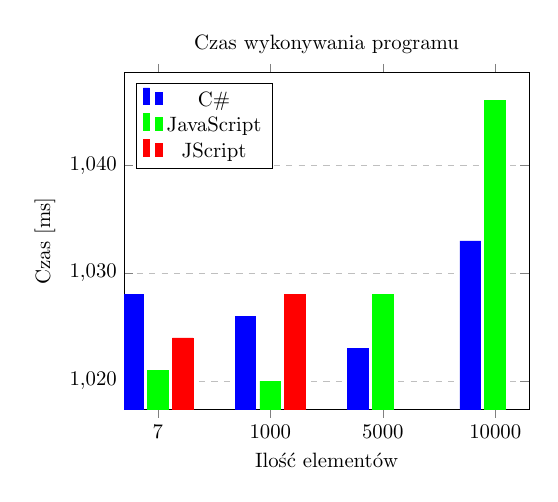
\begin{tikzpicture}[scale=0.75]
    \begin{axis}[
        ybar,
        title={Czas wykonywania programu},
        xlabel={Ilość elementów},
        ylabel={Czas [ms]},
        symbolic x coords={7,1000,5000,10000},
        xtick=data,
        legend pos=north west,
        ymajorgrids=true,
        grid style=dashed,
        % nodes near coords
    ]
    
    \addplot[
        color=blue,
        fill=blue
      ]
      coordinates {
        (7, 1028)
        (1000,1026)
        (5000,1023)
        (10000,1033)
      };
      \addlegendentry{C\#}

      
    \addplot[
      color=green,
      fill=green
      ]
      coordinates {
        (7,1021)
        (1000,1020)
        (5000,1028)
        (10000,1046)
      };
      \addlegendentry{JavaScript}

      
    \addplot[
        color=red,
        fill=red,
      ]
      coordinates {
        (7,1024)
        (1000,1028)
      };
      \addlegendentry{JScript}
        
    \end{axis}
  \end{tikzpicture}
  \caption{Pomiar czasu wykonywania programów dla algorytmu pierwszego.}
\end{figure}

\par Obserwując wyniki pomiarów czasu wykonywania programu, można stwierdzić, że utworzony kompilator jest porównywalny do kompilatora C\#. W przypadku kompilatora JScript różnicę można zauważyć przy większej ilości danych. W przypadku kiedy wektor testowy miał 5000 elementów, czas wykonywania programu zwiększył się średnio o 10 sekund, a w przypadku kiedy wektor testowy posiadał 10000 elementów, czas wykonania osiągną średnio 47 sekund.

\par Kolejnym z kryteriów jest sprawdzenie wykorzystania pamięci dla programów testowych. Zostanie do tego wykorzystane narzędzie \textit{JetBrains dotMemory 2020.2.1}. Test zostanie wykonany dla programów z wektorem wejściowym posiadającym 10000.

\begin{table}[h!]
  \centering
  \begin{tabular}{|l|r|}
  \hline
  Kompilator & Zużycie pamięci \\ \hline
  C\# & 11,26 MB \\ \hline
  JavaScript & 11,25 MB \\ \hline
  JScript & 28,72 MB \\ \hline
  \end{tabular}
\end{table}

\begin{figure}[!h]
  \centering
  \includegraphics[width=0.75\linewidth]{a1_cs_10000.png}
  \caption{Pomiar zużycia pamięci dla algorytmu pierwszego dla kompilatora C\#. Źródło: własne}
  \label{fig:a}
\end{figure}

\begin{figure}[!h]
  \centering
  \includegraphics[width=0.75\linewidth]{a1_js_10000.png}
  \caption{Pomiar zużycia pamięci dla algorytmu pierwszego dla kompilatora JavaScript. Źródło: własne}
  \label{fig:a}
\end{figure}

\begin{figure}[!h]
  \centering
  \includegraphics[width=0.75\linewidth]{a1_jsm_10000.png}
  \caption{Pomiar zużycia pamięci dla algorytmu pierwszego dla kompilatora JScript. Źródło: własne}
  \label{fig:a}
\end{figure}

\newpage
\par Tak ja w poprzednim teście, wyniki pokazują, że pomiędzy programem C\# oraz programem JavaScript nie występuje znaczna różnica. Inaczej jest z programem JScript który zużywa w piku ponad dwukrotnie więcej pamięci.

\par Ostatnim z kryteriów jest zmierzenie wielkości plików skompilowanych programów. Wyniki prezentują się następująco:

\begin{table}[h!]
  \centering
  \begin{tabular}{|l|r|r|r|}
  \hline
  \multicolumn{1}{|c|}{Ilość elementów} & \multicolumn{1}{|c|}{C\#} & \multicolumn{1}{|c|}{JavaScript}& \multicolumn{1}{|c|}{JScript} \\ \hline
  Oryginalne (7)  & 4,00 kB & 3,00 kB & 7,00 kB \\ \hline
  1000            & 15,00 kB & 16,50 kB & 23,00 kB \\ \hline
  5000            & 57,50 kB & 71,00 kB & 89,50 kB \\ \hline
  10000           & 111,00 kB & 139,50 kB & 172,00 kB \\ \hline
  \end{tabular}
\end{table}


\begin{figure}[h!]
  \centering
  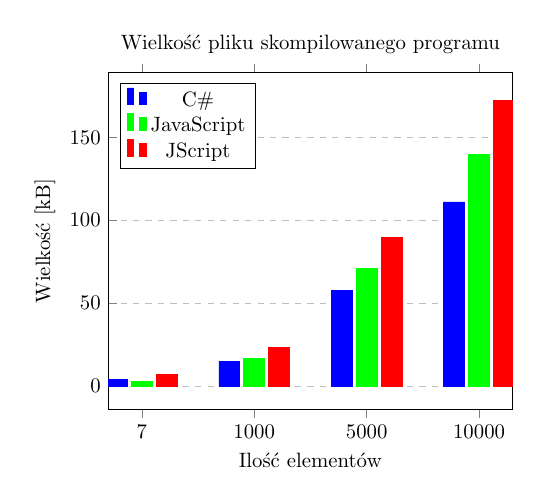
\begin{tikzpicture}[scale=0.75]
    \begin{axis}[
        ybar,
        title={Wielkość pliku skompilowanego programu},
        xlabel={Ilość elementów},
        ylabel={Wielkość [kB]},
        symbolic x coords={7,1000,5000,10000},
        xtick=data,
        legend pos=north west,
        ymajorgrids=true,
        grid style=dashed,
        % nodes near coords
    ]
    
    \addplot[
        color=blue,
        fill=blue
      ]
      coordinates {
        (7, 4.00)
        (1000,15.00)
        (5000,57.50)
        (10000,111.00)
      };
      \addlegendentry{C\#}

      
    \addplot[
      color=green,
      fill=green
      ]
      coordinates {
        (7,3.00)
        (1000,16.50)
        (5000,71.00)
        (10000,139.50)
      };
      \addlegendentry{JavaScript}

      
    \addplot[
        color=red,
        fill=red,
      ]
      coordinates {
        (7,7.00)
        (1000,23.00)
        (5000,89.50)
        (10000,172.00)
      };
      \addlegendentry{JScript}
        
    \end{axis}
  \end{tikzpicture}
  \caption{Pomiar wielkości plików programów dla algorytmu pierwszego.}
\end{figure}

\par Pomiar wielkości plików wskazuje, że stworzony kompilator generuje więcej instrukcji dla programu w porównaniu do kompilatora C\#. Spowodowane jest to słabą optymalizacją generowanego kodu asemblera dla instrukcji. Porównując wielkość programu tworzonego kompilatora do kompilatora JScript, można zauważyć, że wielkość tworzonego pliku wykonywalnego jest mniejsza.


\newpage
\subsection{Algorytm przeszukiwania}

\par Drugim odnalezionym kodem jest algorytm liniowego przeszukiwania tablicy elementów zamieszczonego pod adresem \url{https://www.scriptonitejs.com/javascript-searching-algorithms/}. Kod przedstawia się następująco:

\begin{lstlisting}[language=JavaScript, caption={Algorytm przeszukiwania. Źródło: \url{https://www.scriptonitejs.com/javascript-searching-algorithms/}}, label=alg:alg1]
  var items = [2, 5, 3, 7, 8, 10, 15, 18, 24, 111, 12, 19, 87];
  
  function itemSearch(item) {
      for(var i=0; i < items.length; i++) {
          if(items[i] === item) {
              console.log("Found item " + item + " at index " + i);
              return true;
          }
      }
      //item not found 
      return false;
  }
  
  var item = itemSearch(15);
  if(!item) {
      console.log('Item does not exist!');
  }
\end{lstlisting}

\par Niestety i ten program musiał zostać lekko zmodyfikowany. Modyfikacja polega na przekazaniu wektora testowego \texttt{items} jako argument w funkcji \texttt{itemSearch}. Spowodowane jest to nienajlepsza implementacją zakresu widoczności zmiennych kompilatora. W języku \texttt{JavaScript} jest możliwe odwołanie się do zmiennej zadeklarowanej poza funkcją. Po modyfikacji program prezentuje się następująco:

\begin{lstlisting}[language=JavaScript, caption={Zmodyfikowany kod programu przeszukiwania.}, label=alg:alg1]
  var items = [2, 5, 3, 7, 8, 10, 15, 18, 24, 111, 12, 19, 87];
  
  function itemSearch(items, item) {
      for(var i=0; i < items.length; i++) {
          if(items[i] === item) {
              console.log("Found item " + item + " at index " + i);
              return true;
          }
      }
      //item not found 
      return false;
  }
  
  var item = itemSearch(items, 15);
  if(!item) {
      console.log('Item does not exist!');
  }
\end{lstlisting}

\par Dla powyższego kodu został stworzony odpowiednik dla kompilatora JScript oraz kod został odwzorowany w języku C\#, który prezentuje się następująco:

\begin{lstlisting}[language=CSharp, caption={Odwzorowany kod JavaScript w języku C\# algorytmu przeszukiwania.}, label=alg:alg1]
using System;
using System.Collections.Generic;

namespace dotnet
{
    class Program
    {
        static void Main(string[] args)
        {
            List<int> items = new List<int>() { 2, 5, 3, 7, 8, 10, 15, 18, 24, 111, 12, 19, 87 };
            bool item = itemSearch(items, 15);
            if(!item) {
                Console.WriteLine("Item does not exist!");
            }
        }

        static bool itemSearch(List<int> items, int item){
            for (int i = 0; i < items.Count; i++)
            {
                if(items[i] == item){
                    Console.WriteLine("Found item " + item + " at index " + i);
                    return true;
                }
            }
            return false;
        }
    }
}
\end{lstlisting}

\par Tak jak dla algorytmu pierwszego, testy zostaną wykonane dla oryginalnego wektora wejściowego oraz dla losowo wygenerowanego wektora o wielkościach 1000, 5000 i 10000 składającego się z liczb całkowitych z przedziału od -10000 do 10000. Wyszukiwany element będzie znajdował się w połowie wektora testowego.

\par Algorytm został zbadany pod względem takich samych kryteriów jak algorytm pierwszy. Pierwszym z nich jest zmierzenie czasu wykonywania programu. Wyniki prezentują się następująco:

\begin{table}[!h]
  \centering
  \begin{tabular}{|l|l|l|l|}
  \hline
  Ilość elementów & C\#              & JavaScript       & JScript          \\ \hline
  Oryginalne(13)  & 00:00:01.0156735 & 00:00:01.0262087 & 00:00:01.0222548 \\ \hline
  1000            & 00:00:01.0101172 & 00:00:01.0150919 & 00:00:01.0134737 \\ \hline
  5000            & 00:00:01.0183013 & 00:00:01.0163112 & 00:00:01.0146355 \\ \hline
  10000           & 00:00:01.0167586 & 00:00:01.0116767 & 00:00:01.0203511 \\ \hline
  \end{tabular}
\end{table}

\begin{figure}[h!]
  \centering
  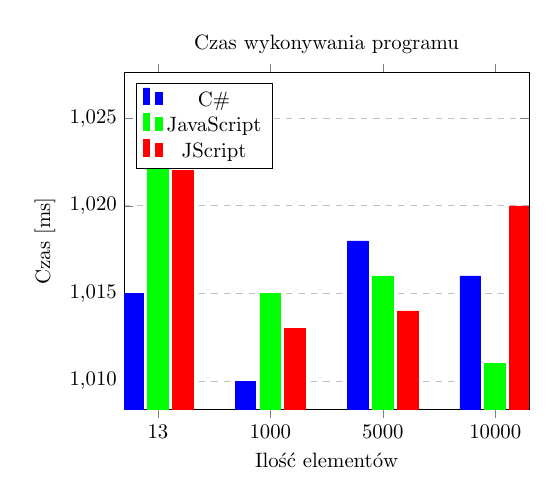
\begin{tikzpicture}[scale=0.75]
    \begin{axis}[
        ybar,
        title={Czas wykonywania programu},
        xlabel={Ilość elementów},
        ylabel={Czas [ms]},
        symbolic x coords={13,1000,5000,10000},
        xtick=data,
        legend pos=north west,
        ymajorgrids=true,
        grid style=dashed,
        % nodes near coords
    ]
    
    \addplot[
        color=blue,
        fill=blue
      ]
      coordinates {
        (13, 1015)
        (1000,1010)
        (5000,1018)
        (10000,1016)
      };
      \addlegendentry{C\#}

      
    \addplot[
      color=green,
      fill=green
      ]
      coordinates {
        (13,1026)
        (1000,1015)
        (5000,1016)
        (10000,1011)
      };
      \addlegendentry{JavaScript}

      
    \addplot[
        color=red,
        fill=red,
      ]
      coordinates {
        (13,1022)
        (1000,1013)
        (5000,1014)
        (10000,1020)
      };
      \addlegendentry{JScript}
        
    \end{axis}
  \end{tikzpicture}
  \caption{Pomiar czasu wykonywania programów dla algorytmu drugiego.}
\end{figure}

\par Wyniki pomiarów czasu wykonywania programu, wskazują nie wielkie różnice czasu pomiędzy kompilatorami jak i pomiędzy różnymi ilościami danych wejściowych.

\par Drugim z kryteriów jest zbadanie wykorzystania pamięci przez programy. Test zostanie wykonany dla programów z wektorem wejściowym posiadającym 10000, oraz element poszukiwany będzie znajdować się w połowie zakresu. 

\begin{table}[h!]
  \centering
  \begin{tabular}{|l|r|}
  \hline
  Kompilator & Zużycie pamięci \\ \hline
  C\# & 10,52 MB \\ \hline
  JavaScript & 10,53 MB \\ \hline
  JScript & 22,36 MB \\ \hline
  \end{tabular}
\end{table}


\begin{figure}[!h]
  \centering
  \begin{minipage}{.48\textwidth}
    \centering
    \includegraphics[width=\linewidth]{a2_cs_10000.png}
    \caption{Pomiar zużycia pamięci dla algorytmu drugiego dla kompilatora C\#. Źródło: własne}
    \label{fig:a}
  \end{minipage}
  \hfill
  \begin{minipage}{.48\textwidth}
    \centering
    \includegraphics[width=\linewidth]{a2_js_10000.png}
    \caption{Pomiar zużycia pamięci dla algorytmu drugiego dla kompilatora JavaScript. Źródło: własne}
   \label{fig:a}
  \end{minipage}
\end{figure}

\begin{figure}[!h]
  \centering
  \includegraphics[width=0.75\linewidth]{a2_jsm_10000.png}
  \caption{Pomiar zużycia pamięci dla algorytmu drugiego dla kompilatora JScript. Źródło: własne}
  \label{fig:a}
\end{figure}

\par Wyniki testu są podobne do wyników testu algorytmu pierwszego. Zużycie pamięci przez program C\# jak i JavaScript jest prawie identyczne. Różnica występuje dla programu JScript, którego zużycie jest ponad dwukrotnie większe.

\newpage
\par Ostatnim z testów jest porównanie zajmowanej przestrzeni dyskowej dla skompilowanych programów. Wyniki prezentują się w następujący sposób:
\begin{table}[!h]
  \centering
  \begin{tabular}{|l|r|r|r|}
  \hline
  Ilość elementów & \multicolumn{1}{l|}{C\#} & \multicolumn{1}{l|}{JavaScript} & \multicolumn{1}{l|}{JScript} \\ \hline
  Oryginalne(13)  & 4,00 kB    & 2,50 kB       & 6,00 kB    \\ \hline
  1000            & 14,50 kB   & 16,00 kB      & 22,00 kB   \\ \hline
  5000            & 57,50 kB   & 71,00 kB      & 88,50 kB   \\ \hline
  10000           & 111,00 kB  & 139,00 kB     & 171,50 kB  \\ \hline
  \end{tabular}
\end{table}

\begin{figure}[h!]
  \centering
  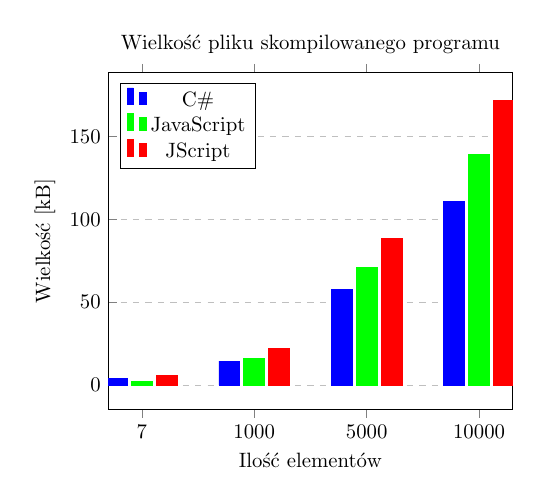
\begin{tikzpicture}[scale=0.75]
    \begin{axis}[
        ybar,
        title={Wielkość pliku skompilowanego programu},
        xlabel={Ilość elementów},
        ylabel={Wielkość [kB]},
        symbolic x coords={7,1000,5000,10000},
        xtick=data,
        legend pos=north west,
        ymajorgrids=true,
        grid style=dashed,
        % nodes near coords
    ]
    
    \addplot[
        color=blue,
        fill=blue
      ]
      coordinates {
        (7, 4.00)
        (1000,14.50)
        (5000,57.50)
        (10000,111.00)
      };
      \addlegendentry{C\#}

      
    \addplot[
      color=green,
      fill=green
      ]
      coordinates {
        (7,2.50)
        (1000,16.00)
        (5000,71.00)
        (10000,139.00)
      };
      \addlegendentry{JavaScript}

      
    \addplot[
        color=red,
        fill=red,
      ]
      coordinates {
        (7,6.00)
        (1000,22.00)
        (5000,88.50)
        (10000,171.50)
      };
      \addlegendentry{JScript}
        
    \end{axis}
  \end{tikzpicture}
  \caption{Pomiar wielkości plików programów dla algorytmu pierwszego.}
\end{figure}

\par Wyniki pomiarów są podobne jak w przypadku pomiarów algorytmu pierwszego. Wraz z zwiększeniem ilości elementów wektora wejściowego, pliki wykazują coraz większą różnicę zajmowanego miejsca na przestrzeni dyskowej.
